\documentclass{report}
\usepackage{color}
\usepackage[utf8x]{inputenc}
\usepackage[T1]{fontenc}      % caractères français
\usepackage{geometry}         % marges
\usepackage[francais]{babel}  % langue
\usepackage{graphicx} 
\usepackage{wrapfig}
\usepackage{listingsutf8}
\usepackage[final]{pdfpages} 

\usepackage{amsmath}
\usepackage{enumitem}     % images
\usepackage{verbatim}         % texte préformaté
\title{\LARGE Implémentation d'un outil de veille concurrentielle concernant des articles de loisirs sportifs}      % renseigne le titre
\author{Clément BALESTRAT - Nicolas KERMARC - Yann PRAVOSSOUDOVITCH}
          
\pagestyle{headings}          % affiche un rappel discret (en haut à gauche)
                         % de la partie dans laquel on se situe
                         
\makeatletter
\def\thetitle{\@title}
\def\theauthor{\large\@author}
\def\thedate{\@date}
\makeatother
\definecolor{light-gray}{gray}{0.95}
\lstset{backgroundcolor=\color{light-gray}, inputencoding=utf8/latin1}
\begin{document}
\begin{titlepage}


\includegraphics[scale=0.1]{logo.jpg} 

\centering
\vfill
{\Huge\bfseries \thetitle}
\vskip 1cm
{\Large \theauthor}
\hspace{10.5cm}
\vskip 0.25cm
\Large Rapport technique du Projet Industriel de Fin d'Etudes\\
\Large Département Informatique et Gestion
\vskip 0.25cm
\Large 25 janvier 2013
\vskip 0.5cm
\vfill
\large Tuteur: Anne-Laure De Lauzun
\hspace{2cm}
\large Demandeur: Sébastien BERNIS
\end{titlepage}



\renewcommand{\contentsname}{Sommaire}
 


\tableofcontents

\chapter{Introduction}
Ce présent rapport vient en complément du rapport de synthèse du projet industriel de fin d'études mené par Balestrat Clément, Kermarc Nicolas et Pravossoudovitch Yann durant PIFE en 5ème année de l'école Polytech' Montpellier.\\\\
Il décrit les différentes phases du développement au niveau technique ainsi que les choix établis tel que le langage et les outils utilisés qui nous ont permis d'arriver au logiciel final.\\\\
Nous retrouverons par exemple des détails sur les options prises pour créer un algorithme permettant de récupérer la plupart des articles des différents sites ciblés ainsi que de les faire correspondre entre eux.\\\\
Nous présenterons au cours de ce rapport le choix des technologies tel que le langage, les librairies, le type de base de données ou encore les outils. Nous verrons par la suite comment nous sommes arrivés à réaliser ces algorithmes dont nous regarderons le temps d'éxécution en passant par le choix de l'architecture du programme. Enfin, nous nous intéresserons à la partie graphique de la solution que le client utilisera.

\chapter{Choix des technologies}
\section{Les langages}
Nous aurions pu choisir le langage Python ou même C pour effectuer ce travail, puisqu'il sont rapides, efficaces et qu'il peuvent s'exécuter sur un serveur dédié. Mais le driver MongoDB (type de base de données que nous étudierons plus bas) n'est pas bien géré sur ces langages où plutôt, est très bien géré avec PHP.\\\\
Nous nous sommes donc plutôt tournés vers le langage PHP car il est simple d'utilisation et qu'il permet de tester les fonctionnalités plus rapidement puisque c'est un langage script, donc non compilé. De plus la librairie pour la base de données de type Mongo est assez facile d'utilisation et bien qu'il n'y ai pas une grande communauté d'utilisateurs, les porteurs du projet peuvent mettre à disposition leurs connaissances.\\\\
Pour ce qui est des données à traiter, nous avons utilisé une librairie DOM qui permet d'accéder au contenu des différentes pages articles des sites webs pour en récupérer le prix et le libellé entre autres.
Nous détaillerons l'utilisation de cette librairie dans le prochain paragraphe.\\
L'objectif initial est de faciliter l'échange automatisé de contenus complexes.\\
Voici un exemple du fichier XML utilisé pour ce projet afin de mieux comprendre comment l'utiliser.\\\\
Pour la partie graphique, NICO
~\\

\section{La base de données Mongo}
Nous avons décidé d'utiliser MongoDB pour la conception de base de données car elle correspond a l'utilisation que nous voulons en faire.\\
MongoDB ( de "hu\textbf{mongo}us" signifiant gigantesque) est une base de données open-source NoSQL (pour "Not only SQL") qui est évolutive et de haute performance.\\\\
MongoDB permet de ne pas faire de requêtes SQL, on parle alors de base SchemaLess ou dite orienté Documents.
La première grande utilité est qu'on est pas obligé d'avoir des scripts de migration pour définir et faire évoluer le format de sa base de données. C'est simple : on crée son objet et on le met dans notre base. Cette logique est donc beaucoup plus orientée Objet Dynamique.\\
Ceci est donc bien plus efficace lorsque l'on veut gérer un nombre important de data.\\\\
On va ici expliquer le fonctionnement et les avantages de celui-ci couplé au langage de programmation PHP.
En effet quelques lignes de code, tel que l'exemple ci-dessous, sont nécessaires pour pouvoir utiliser une base de données MongoDB.
\begin{lstlisting}
$m = new Mongo(); // Connexion a Mongo etablie.

// Choix de la base de donnees.
$db = $m->selectDB("comparator");

// Collection des articles de la base de donnees.
$articles = $db->articles->find();
\end{lstlisting}
~\\
Ces 3 lignes de codes permettent la connexion à la base de données MongoDB se nommant "comparator".\\
La variable \$articles contient, après exécution, la totalité des articles de la BDD avec tous ces attributs sous forme d'un tableau PHP.\\\\
Pour faire des requêtes sur la base de données tel que obtenir la liste des articles d'un site, c'est d'une grande facilité:
\begin{lstlisting}
// Tous les articles du site ayant pour id $IDSite
$articlesSpec = $db->articles->find(array('_id' => new MongoId($IDSite)));
\end{lstlisting}
~\\
Nous pouvons également insérer des éléments en base avec une grande facilité.
\begin{lstlisting}
$articleToAdd = array(
			"url" => $urlArticle,
			"name" => $name,
			"img" => $img, 
			...
		);
$articles->insert($articleToAdd);
\end{lstlisting}
Nous pouvons constater ici que nous créons un array contenant tous les attributs nécessaires et que nous l'insérons simplement en base grâce à la fonction insert().

\section{Les outils}
\subsection{Github}
Une fois que nous avons décidés comment faire ce projet, il nous fallait pouvoir l’envoyer pour qu’il soit utiliser. Nous avons alors mis en place un dépôt Git sur le site Github.com. \\
Il bénéficie de fonctionnalitées indispensables tel qu’un système de contrôle de versions décen- tralisé. Celui-ci nous a sorti plusieurs fois de situations pénibles puisqu’il archive toutes les versions du projet sur son site et ainsi nous avons pu revenir à une version antérieur non buguée.
\begin{figure}[h]
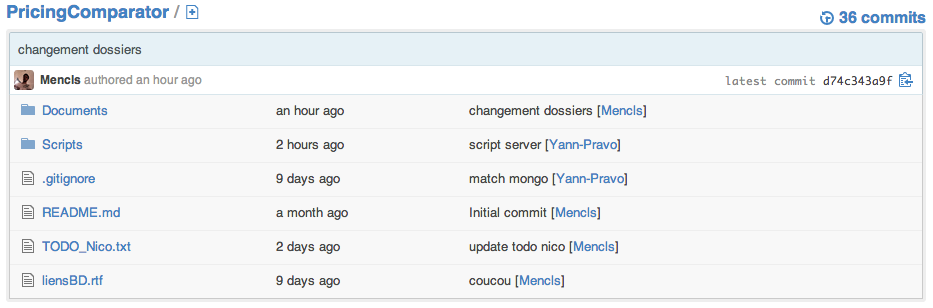
\includegraphics[scale = 0.5]{./img/github.png}
\caption{PricingComparator Repo}
\end{figure}

\subsection{OVH}
OVH est un hébergeur qui proposent des serveurs dédiés, des serveurs privés, de l'hébergement mutualisé, etc.\\
Nous avons décidés, avec le demandeur, d'opter pour un serveur dédié fonctionnant sous Ubuntu Server 12.04 "Precise Pangolin" LTS. Cette distribution — basée sur un système 64bits — nous permet non seulement d'héberger et de déployer notre projet pour qu'il soit utilisable n'importe où, mais il nous offre également une puissance de calcul bien supérieur à celle de nos ordinateurs personnels. On verra plus tard que ce dernier point est très important puisque car le temps d'éxécution des algorithmes est conséquent.

\subsection{LaTeX}
Pour la rédaction des rapports, nous avons décidé d'utiliser le repo github pour partager les rapports.\\
Nous avons décidés de les écrire dans le langage LaTeX qui est un système de composition de documents. Il est devenu la méthode privilégiée d'écriture de documents techniques et scientifiques puisqu'il permet un rendu simple, épuré, mais très efficace.\\
Ce présent rapport technique ainsi que le rapport de synthèse sont écrits en LaTeX.

\chapter{Back-End}
\section{Structure de la BDD}
Dès le début, nous avons décidés d'avoir une collection Sites contenant une id, un nom et une url ainsi qu'une autre Articles contenant une id une url, l'id du site correspondant, un nom et un prix.
Cette structure était relativement bonne mais plusieurs contraintes se sont présentées.\\
\paragraph{}
Tout d'abord, le demandeur a fait la requête d'avoir une courbe d'évolution du prix dans le temps or notre structure ne le permettait pas. Nous avons alors décidé de remplacer le simple attribut float "Prix" par un tableau d'éléments comprenant un prix et une date.\\
De plus, nous avons jugés qu'ajouter un attribut catégorie pour les articles facilitait grandement la tâche des scripts et permettait de pouvoir faire un affichage par catégorie dans le front-end. Nous avons alors décidé d'ajouter cet attribut à la collection articles ainsi qu'à la collection Sites sous forme d'un tableau comprenant le nom de toutes les catégories du site, son nom commun aux sites, ainsi que son url respective.\\\\
Voici la structure finale de notre solution:
\begin{lstlisting}
Sites :	"_id" => MongoID,
	"name" => String,
	"url"  => String,
	"category" => Array(
				"name" => String,
				"commonName" => String,
				"url" => String )
\end{lstlisting}
\newpage
\begin{lstlisting}							
Articles : "_id" => MongoID,
	   "name" => String,
	   "url"  => String,
	   "_site" => MongoID,
	   "category" => String,
	   "prices"	=> Array(
				"price" => float,
				"date" => MongoDate )
\end{lstlisting}

\section{Récupération des articles}
L'une des parties les plus délicates et contraignantes de ce projet à été tout d'abord de récupérer le plus d'articles possibles sur les différents sites de plongée.\\
En effet, nous nous sommes trouvé face à de nombreux problèmes, notamment comment automatiser cette récupération pour tous les articles et comment faire face au besoin de mémoire important de l'algorithme?\\\\
Pour ce faire, nous avons utilisé une librairie DOM —Document Object Model— php : SimpleHTMLDom.\\

Le SimpleHTMLDom est une librairie écrite en PHP5 qui permet de manipuler du HTML très facilement. Il fonctionne en s'appuyant sur les balises des pages HTML.\\
Les objets des articles tel que le prix, le libellé ou encore l'url de l'image peuvent être retrouvés en utilisant des sélecteurs — comme en JQuery ou XML — pointant vers l'id, la classe, les tags et bien d'autres choses.\\\\
Exemple d'utilisation: \\
\begin{lstlisting}
// Recupere le fichier html de la page de l'article
$html = file_get_html("url de l'article");

// Recupere la classe title
// ->plaintext ne prend en compte que le contenu
$nomArticle = $html2->find('.title', 0)->plaintext;
\end{lstlisting}

On a donc utilisé pour chaque site, les DOM correspondants aux pages articles afin de récupérer les données que l'on utilisera plus tard tel que le libellé, le prix, la photo de l'article, etc.\\\\
Beaucoup de problèmes ont étés rencontrés ici puisque selon les sites webs, un manque de rigueur était notable sur le code de ceux-ci.\\\\
Pour automatiser ce processus sur tous les articles de tous les sites, nous avons décidés de découper le site en catégories (Combinaisons, Palmes, Masques, ...) pour ensuite les parcourir sur plusieurs niveaux jusqu'à arriver sur les pages articles. Ceci est possible grâce aux crawlers créé par nos soins, en utilisant encore une fois la libraire DOM.
\begin{lstlisting}
$html = file_get_html($url);
	$categ = $html->find('.category_child_listing h3.bp_product_name');
	foreach ($html->find('.h3.bp_product_name') as $a1) {
\end{lstlisting}

Nous avons à ce stade rencontré un problème de mémoire et avons eu des erreurs de segmentation car les quantitées de données enregistrés étaient trop importants. Après de nombreuses recherche, on a découvert que la librairie DOM était tout simplement composée d'une fonction permettant de libérer la mémoire.
\begin{lstlisting}
$html->clear();
unset($html);
\end{lstlisting}

Une fois ces informations récupérés donc, on a besoin de l'enregistrer en base de données pour pouvoir les utiliser plus tard.\\
On crée donc un array pour chaque article avec toutes ces informations que l'on insère en base très facilement grâce au driver mongo:\\
\begin{lstlisting}
$array_article = array(
			"url" => $urlArticle,
			"_site" => new MongoId($idSite),
			"category" => $cat,
			"name" => str_replace("\t", "", $name),
			"img" => $img,
			"match" => array(),
			"prices" => array(array(
				"price" => (float) $prixArticle,
				"time" => new MongoDate())));
			
$db->articles->insert($array_article);
\end{lstlisting}

On remarque ici qu'à chaque ajout, un tableau avec le prix de l'article ainsi que la date d'éxécution de l'algorithme est ajouté. Ce tableau sera rempli ensuite grâce à un autre algorithme qu'on lancera périodiquement pour avoir une courbe de l'évaluation de chaque article.

\section{Mise à jour du prix}
En ce qui concerne l'ajout du prix avec sa date, nous avons créé un autre script qui prend comme argument l'id du site de l'article, son id, et son url. On va ensuite directement sur la page de l'article pour récupérer le prix et l'ajouter dans le tableau prices de l'article en question.
\begin{lstlisting}
$array_price = array("price" => $price, "time" => new MongoDate());

$db->articles->update(array(
		"_id" => new MongoId($idArticle)),
		array('$push' => array('prices'=> $array_price)));
\end{lstlisting}
Ici, c'est la fonction mongo push qui permet d'ajouter l'array contenant le prix et la date d'éxécution de l'algorithme au tableau correspond, présent dans la base de donnée.
\newpage

\section{Matching}
L'algorithme de matching est l'une des parties les plus importantes du back-end. Il permet de faire correspondre les articles entre les différents sites web. On compare ici tous les articles d'un site avec ceux des autres sites.\\
On compare ici les libellés des articles dont on aura auparavant enlever les accents et mis en minuscule grâce à la fonction minusculesSansAccents(\$libelle). Les libellés sont mis sous forme de tableaux de mots, on compare ensuite ceux-ci avec ceux du libellé de l'article comparé. Un mot est accepté comme matché lorsque l'on trouve un mot similaire à 90\% dans le tableau que l'on compare grâce à la fonction php similar\_text(\$Word1, \$Word2, \$percent);\\
Si le libellé contient plus de 5 mots, au moins 3 mots doivent matcher avec ceux de l'article comparé pour être accepté, sinon, deux mots suffisent.\\
Le prix rentre aussi en compte dans la comparaison des articles, seul les articles dont les prix ne diffèrent pas de plus de 25\% peuvent être matchés entre eux.
\begin{lstlisting}
if (arrayCompare($mots1, $mots2) >= $compteur
	&& ($prix1 >= $prix2 - $prix2*0.25
	&& $prix1 <= $prix2 + $prix2*0.25))
{
	$nbMatch++;
}
\end{lstlisting}

Lorsqu'un article est matché avec un autre article d'un autre site, on ajoute l'id de ce dernier dans un tableau 'match' de l'article en question.
\begin{lstlisting}
$db->articles->update(array(
			"_id" => new MongoId($art['_id'])),
			array('$push' => array(
				'match'=> new MongoId($artComp['_id']))
			));          
\end{lstlisting}

On aura donc pour chaque article, une liste d'articles des autres sites qui pourrait correspondre. On validera ensuite le matching en graphique, dans la partie front-end.
\newpage

\section{Temps d'éxécution}
Une des plus grandes difficultées de ce projet est de ne pas avoir un temps d'éxécution trop important car la quantité de donnée à gérer est très important.\\
L'algorithme de récupérations des articles permet d'enregistrer plus de 9000 articles, ce qui prends beaucoup de temps. De plus, les sites webs sur lesquels nous récupéront les articles ne sont pas toujours des plus rapides ce qui ralentit encore plus l'éxécution.\\
\begin{figure}[h]
\begin{center}
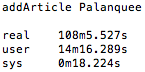
\includegraphics[scale = 0.7]{./img/palanquee1.png}
\caption{Temps d'éxécution de l'algo de récupération d'articles pour le site de la Palanquee}
\end{center}
\end{figure}
On voit ici que la récupération des articles pour un site prend environ 1h50 ce qui est tout à fait acceptable car la fréquence d'éxécution de cet algorithme n'est pas grande.\\\\
Ce temps d'éxécution est réduit grâce au serveur OVH de quelques dizaine de minutes. Cet écart n'est pas plus important à cause de la lenteur des sites webs crawlés.\\
\begin{figure}[h]
\begin{center}
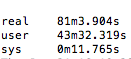
\includegraphics[scale = 0.7]{./img/palanquee2.png}
\caption{Temps d'éxécution de l'algo sur le serveur OVH}
\end{center}
\end{figure}

L'algorithme de mise à jour des prix est lui bien plus rapide bien que son temps d'éxécution est étroitement lié avec la rapide du site web sur lequel il se trouve. On peut alors récupérer le prix d'un article sur un site en environ 1 seconde.\\\\

C'est sur l'algorithme de matching qu'il est intéressant de regarder la différence du temps d'éxécution entre nos ordinateurs personnels et le serveur. Ce temps d'éxécution est très grand de base et exponentiel. En effet, il faut comparer environ 4 mots (taille du libellé d'un article) avec 4 mots d'un libellé d'un autre article fois le nombre d'articles restant dans la base de données qui est de plus de 7000.\\
On arrive donc a un temps d'éxécution d'environ 2 heures pour matcher les produits d'un site web. Il est également correct puisque lancer avec la même périodicité que l'algorithme de récupérations des articles.\\
Ce temps d'éxécution est diminué de 30\% grâce au serveur OVH ce qui nous permet, avec tous les sites, d'économiser plusieurs heures de calcul.

\chapter{Front-End}

\section{Une application “single page app”}
L'application que nous avons réalisée a été construite dans une philosophie d'application page unique. C'est à dire qu'en fait, le seul backend que nous avons est une API qui renvoie du JSON. Tout est ensuite traité côté client avec le framework AngularJS. De plus, lors d'un changement de page, ce n'est pas le serveur qui répond à l'URL donnée mais le client qui simule un changement d'URL grâce au HTML5 PushState.

\subsection{API : NodeJS et MongoJS}
NodeJS fut un choix qui coule de source puisqu'il a été construit sur le même moteur JavaScript (V8) que MongoDB. De plus, les documents sous MongoDB sont accessbiles au format JSON qui est bien sûr le format de base pour les Objets javascript. Aucune serialisation/désérialisation à faire, puisque les données qui nous proviennent de notre BD sont déjà au bon format et exploitables par notre backend.\\

NodeJS permet donc d'écrire du JavaScript côté serveur. Celà peut paraître étrange mais à l'heure actuelle la communauté Node explose, et il a l'avantage d'être single-threaded MAIS asynchrone, c'est à dire qu'il n'y a -quasiment- pas de fonctions bloquantes. Ainsi par exemple, si on a une grosse requête en BD à faire, on peut continuer à servir des requêtes HTTP sans faire attendre les clients; puisque la requête est traitée de manière asynchrone, en “fond”.\\\\

Nous avons utilisé Express qui est le framework le plus répandu pour NodeJS et qui permet de créer un service Web très rapidement.\\

Express nous permet de :\\
- Servir notre application (répondre aux requêtes sur l'URL du service et renvoyer nos fichiers HTML, CSS, etc...)\\
- Servir notre API, sur des URL prefixées par /api\\\\

La seule difficulté de NodeJS et la courbe d'apprentissage initiale. Puisqu'il s'agit d'un langage asynchrone, il faut toujours fournir une fonction de rappel qui sera donc appellée lorsque la fonction aura finit son éxécution.\\

Cela peut ainsi paraître troublant de savoir que si on écrit ce code

\begin{lstlisting}	
var requete = requeteSQL('ma requete...');
echo 'Requete effectuee'
\end{lstlisting}

Le texte “requête effectuée” va s'afficher avant que la requête soit terminée...\\
Ainsi en NodeJS on va plutôt écrire ce genre de code :
\begin{lstlisting}
var requete = requreSQL('ma requete...',function(data) {
   echo 'Requete terminee!'
   echo data;
});
\end{lstlisting}

Il faut donc un petit temps d'adaptation et d'apprentissage puisqu'évidemment les langages asynchrones sont plutôt rares et nous sommes en général habitués à travailler sur des environnements multi-threadés mais synchrones.\\\\

Nous avons utilisé MongoJS qui est un wrapper pour le driver natif MongoDB pour Node. MongoJS fournit une API qui est totalement similaire à l'API MongoDB sous Terminal. On va écrire en Node exactement les mêmes requêtes qu'on ferait dans le shell Mongo, ce qui est plutôt agréable et permet d'unifier tout le rapport avec la BD.
\newpage

\subsection{Front-end : AngularJS}
AngularJS est un framework sponsorisé par Google qui est actuellement très en vogue dans le monde des applications Web. En fait, si HTML avait été pensé pour développer des applications Web dynamiques, cela aurait été Angular.

Angular permet d'ajouter une structure de type MVC a notre application, tout en nous permettant de développer rapidement et d'avancer vite grâce à son API simplifiée et ses directives.\\

Voici par exemple un exemple du Routeur de notre application, qui parle de lui-même, et qui permet simplement de choisir le bon controlleur et la bonne vue HTML à afficher en fonction de l'URL demandée.

\begin{lstlisting}
var comparatorAngularApp = angular.module('comparatorAngularApp', [])
  .config(['$routeProvider', function($routeProvider) {
    $routeProvider
      .when('/', {
        templateUrl: 'views/main.html',
        controller: 'MainCtrl'
      })
      .when('/validation',
        templateUrl:'views/validation.html',
        controller:ValidationCtrl
      })
      .otherwise({
        redirectTo: '/'
      });
  }]);
\end{lstlisting}

Ainsi en quelques lignes de code on peut déjà définir un comportement à notre application et séparer clairement ses différentes parties.\\

De plus, Angular propose un modèle appellé “Two ways data binding”. Cela veut dire que si une variable présente dans un controlleur est modifiée sur le template (par un input text), alors la variable sera aussi rafraichie côté JavaScript, et inversement.\\

Template HTML :
\begin{lstlisting}
<div ng-repeat=\"currentArticle in articles'\">
  <a href='' ng-click='getMoreInfos(currentArticle)'>
  	{{currentArticle.name}}</a>
</div>
\end{lstlisting}
\newpage
Controlleur :
\begin{lstlisting}
$scope.articles = [
   { name : 'Ordinateur de plongée', infos:'Un très bon ordi' },
   { name: 'Tuba', infos:'Peut permettre de respirer sous l'eau' }
];
$scope.getMoreInfos = function(article) {
  alert('Voici plus d'infos : '+article.infos);
}
\end{lstlisting}

En a peine quelques lignes de code et quelques instructions HTML qui sont très compréhensibles, nous pouvons déjà avoir une application dynamique ET structurée. 

\paragraph*{Interface}
Nous avons utilisé Twitter Bootstrap qui est à l'heure actuelle la référence en terme de framework CSS. Avec une communauté énorme et un design simple et efficace, Bootstrap a déjà été adopté par des dizaines de milliers de WebApp. Bootstrap permet notamment aux développeurs (qui sont rarement designers) de développer des applications sans négliger l'aspect, et ce, sans avoir aucune base en design ni en intégration CSS (ou presque).

\subsection{Un seul langage}
L'immense avantage de nos choix  technologiques et que nous avons un seul et même langage, que ce soit pour le Front-end ou pour le Back-end : JavaScript. Cela est donc évidemment un gros atout puisqu'il n'y a pas de “conversion” à faire, les petites erreurs sont moins fréquentes... Et la progression est plus rapide!

\subsection{Workflow}
Nous avons utilisé Yeoman qui est un utilitaire en ligne de commande développé par Google. Yeoman permet d'accélérer le processus de développement des webapp ainsi que leur workflow. Ainsi, toutes les tâches répétitives et ennuyantes telles que la minification, la compression des fichiers JavaScript et autres sont prises en compte automatiquement par Yeoman.\\

Par exemple, dès qu'on change un fichier de l'application, la page web se rafraîchira toute seule pour refléter les modifications effectuées (sous Google Chrome en tout cas).

\chapter{Tests}
En ce qui concerne le front-end, nous avons utilisé Testacular qui est fournit avec angular. Cet outil permet d'écrire des tests 'end to end'.
\begin{lstlisting}
describe('PhoneCat controllers', function() {
  describe('PhoneListCtrl', function(){
    var scope, ctrl;
 
    beforeEach(function() {
      scope = {},
      ctrl = new PhoneListCtrl(scope);
    });
    
    it('should create "phones" model with 3 phones', function() {
      expect(scope.phones.length).toBe(3);
    });

    it('should set the default value of orderProp model', function() {
      expect(scope.orderProp).toBe('age');
    });
  });
});
\end{lstlisting}
\newpage

Pour la partie back-end, nous avons écrits des tests permettant de vérifier que que les informations étaient non seulement bien inscris dans la base mongo mais aussi que les informations étaient correctes.\\
\begin{figure}[h]
\begin{center}
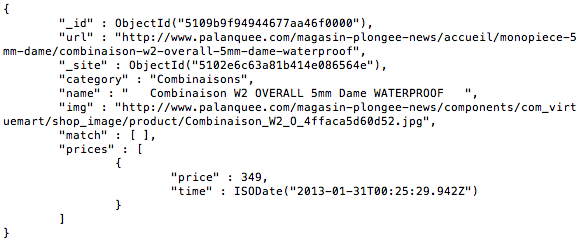
\includegraphics[scale = 0.7]{./img/article.png}
\caption{Article en base}
\end{center}
\end{figure}

\chapter{Manuel d'utilisation}
Les algorithmes sont tous lancés de automatiquement et périodiquement, en revanche on peut les utiliser de manière manuel. La mise à jour du prix peut être lancé pour un article graphiquement directement sur notre site web.\\
On peut en revanche le lancer manuellement.
\begin{lstlisting}
// usage :
crawlerArticle [idSite] [idArticle] [urlArticle]

// exemple sur un article de la Palanquee :
crawlerArticle 5102e6c63a81b414e086564e 5109b9f94944677aa46f0000
	http://www.palanquee.com/magasin-plongee-news/accueil/monopiece
	-5mm-dame/combinaison-w2-overall-5mm-dame-waterproof
\end{lstlisting}

La récupération d'article se lance comme suit, il faut exécuter ce script pour toutes les catégories de tous les sites.
\begin{lstlisting}
usage :
crawlerCateg [idSite] [nomCategorie] [urlCategorie]

// exemple sur la categorie Gants de la Palanquee :
crawlerArticle 5102e6c63a81b414e086564e 'Gants'
	'http://www.palanquee.com/magasin-plongee-news/accueil/gant'
\end{lstlisting}

Pour éxécuter le matching, il suffit simplement de lancer le script avec l'id du site web souhaité.
\begin{lstlisting}
// usage :
matching [idSite]

// exemple avec la Palanquee :
matching 5102e6c63a81b414e086564e
\end{lstlisting}

\chapter{Conclusion}
Ce projet réalisé en collaboration fut très enrichissant. Nous avons été confronté à certaines contraintes professionnelles comme les délais, la gestion du travail en équipe, la gestion de la mémoire etc.\\\\
Nous avons également amélioré nos compétances technique grâce à l'utilisation de nouveaux outils tel que les crawlers de sites.\\\\
Nous avons beaucoup appris sur la gestion d’un projet informatique. Gérer un projet ne signifie pas seulement analyser les besoins et concevoir l’outil informatique, mais prendre en compte de nombreux facteurs. Par exemple, il faut respecter un planning des tâches, prendre des décisions en accord avec la maîtrise d’ouvrage, élaborer et proposer une interface graphique conviviale. Ce projet a été de notre point de vue une réussite bien qu'il reste encore de la place pour améliorer le logiciel tel qu'une partie facturation ou encore un ajout automatique d'autres sites webs.

\chapter{Glossaire}
\begin{description}
\item[SGBD] est un logiciel système destiné à stocker et à partager des informations dans une base de données, en garantissant la qualité, la pérennité et la confidentialité des informations, tout en cachant la complexité des opérations.
\item[NoSQL] désigne une catégorie de système de gestion de base de données (SGBD) destinés à manipuler des bases de données géantes pour des sites web de très grande audience tels que Google, Amazon.com, Facebook ou eBay. Cette catégorie de produits fait le compromis d'abandonner certaines fonctionnalités classiques des SGBD relationnels au profit de la simplicité et de la performance.
\item[une collection] est l'équivalent d'une table en NoSQL, sauf qu'il n'est pas nécessaire d'avoir un schéma fixe pour tous les éléments.
\item[Crawler] Un robot d'indexation est un programme qui explore un site web et permet d'en récupérer des informations.
\item[PHP] (Hypertext Preprocessor) est un langage de scripts libre principalement utilisé pour produire des pages Web dynamiques via un serveur.
\item[HTML] (Hypertext Markup Language) est le format de données conçu pour représenter les pages web.
\item[CSS] (Cascading Style Sheets) est un langage informatique qui sert à décrire la présentation des documents HTML et XML. 
\item[MongoDB] est un système de gestion de base de données orientée documents, libre, montant bien en puissance (scalable), à performance raisonnable, ne nécessitant pas de schéma prédéfini des données.

\end{description}
\end{document}